\documentclass[11pt,a4paper,utf8]{article} 
\usepackage{fontspec}
\setmainfont{Times New Roman}    

\usepackage{abstract} 
\usepackage{amsmath}  
\usepackage{authblk}
\usepackage{array} 
\usepackage{booktabs} %绘制表格  
\usepackage{biblatex} 
\usepackage{caption2} %标题居中
\usepackage{color} 
\usepackage{colortbl}
\usepackage{ctex}
\usepackage{enumerate}  
\usepackage{float}
\usepackage{fontspec}
\usepackage{geometry} 
\usepackage{graphicx}  
\usepackage[hidelinks]{hyperref}
\usepackage{listings} 
\usepackage{longtable} 
\usepackage{multirow}
\usepackage{biblatex}
\usepackage{subfigure}
\usepackage{soul}
\usepackage{titlesec}  
\usepackage{fancyhdr} % 导入fancyhdr包
\usepackage{ulem} 

\geometry{a4paper, left=2.5cm, right=2.5cm, top=2.5cm, bottom=2.5cm}%设置页面尺寸
\lstset{
		numbers=left, %设置行号位置
		numberstyle=\tiny, %设置行号大小
		keywordstyle=\color{blue}, %设置关键字颜色
		commentstyle=\color[cmyk]{1, 0, 1, 0}, %设置注释颜色
		escapeinside=``, %逃逸字符(1左面的键), 用于显示中文
		breaklines, %自动折行
		extendedchars=false, %解决代码跨页时, 章节标题, 页眉等汉字不显示的问题
		xleftmargin=1em, xrightmargin=1em, aboveskip=1em, %设置边距
		tabsize=4, %设置tab空格数
		showspaces=false %不显示空格
}

\pagestyle{fancy} 
\fancyhead[L]{}
% 页脚设置
\fancyfoot[C]{\thepage} % 页码 
\renewcommand{\footrulewidth}{1pt} 
\begin{document}  
\pagenumbering{arabic} %设置数字页码  

\section{一些想法}
\begin{itemize}
    \item 某个人的微博分析:LDA 主题聚类、情绪分类等;
    \item \sout{社交网络分析:基于 PageRank算法的关键人物定位、群体画像等}
    \item 评论者感情倾向分析、发言意愿
    \item 可以来一些舆情事件,然后用一个主题串起来 
\end{itemize}   
   
\subsection{百度指数}
里面有:
\begin{itemize}
    \item 趋势研究:搜索指数、搜索指数概览、资讯关注
    \item 需求图谱:需求图谱、相关词热度
    \item 人群画像:地域分布、人群属性、兴趣分布
\end{itemize} 
还有行业排行
 
\subsection{情感倾向分析}
首先对抓取的舆情数据进行分词处理,然后结合情感语料数据库和情感分析算法对切分后的语料进行情感计算、分析,并进行情感标注。通过聚类和分类得出个体情感倾向和群体情感倾向,以便进一步发现个体情感异常和群体情感异动。 
\begin{figure}[H]
    \centering
    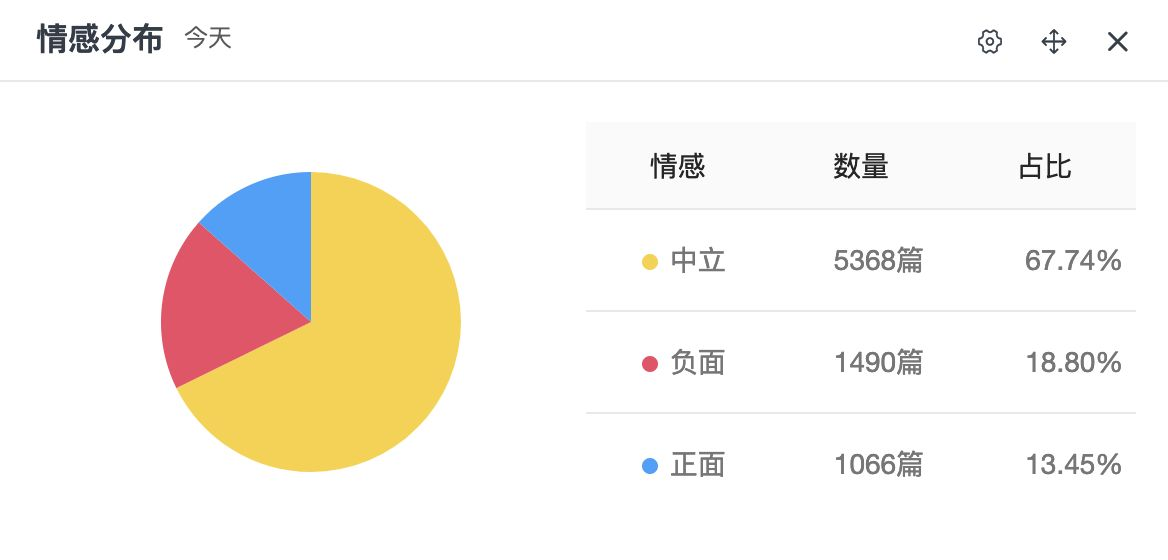
\includegraphics[width=10cm,height=6cm]{images/情感分布.jpg}   
\end{figure}  

\subsection{舆情风险评价}
对网络信息发布者进行用户画像,包括年龄、性别、地域、使用终端等信息,用户画像便于对高舆情风险人群进行动态跟踪监视; 建立风险评价指标体系、风险评价模型,根据动态舆情数据,对事前舆情隐患风险、事中舆情恶化风险以及事后舆情衍生风险进行评价,并适时给出舆情风险预警。

\subsection{趋势分析预测}
通过对采集到的时序网络舆情数据运用线性回归分析、决策树回归分析、隐马尔可夫预测、深度学习等方法进行回归预测分析,可给出网络舆情的演变趋势,为风险预警和处置决策提供参考。

\subsection{微博评论}
时间维度:舆情的热度时间趋势 \\ 
空间维度:舆情的地理分布 \\
传播维度:舆情的传播情况,从哪里来,话题的演变, \\
主题维度:主要议题,议题与网民固有诉求的呼应等 \\
情感维度:网民支持还是反对,还是一半支持一半反对。 \\
每一个维度都可以做的很深刻。譬如传播,既可以简单的写先从朋友圈传播到微博,又从微博迅速扩散到各大舆论场。又可以建模分析,譬如超网络传播模型之类的。

\subsection{预测}
传播图谱 \\ 
不同的舆论场有不同的传播模型。预测的话其实掌握主流舆论场的传播模型,再结合议题属性和舆论场的属性,就可以做出不错的预测了。

\subsection{舆情分析网站}
 
\subsubsection{第谷搜索}
http://www.digudata.com/ 这个可以付费下载微博数据

\subsubsection{海量信息}
http://hailiangxinxi.com/ \\ 
这个网站的介绍可以看这个:https://zhuanlan.zhihu.com/p/338912325

\subsubsection{蚁坊软件}
https://www.eefung.com/ \\  

\subsubsection{识微科技}
https://www.civiw.com/ \\ 

\subsubsection{百度舆情检测}
http://yuqing.baidu.com/saas/intro/newindex \\
\textbf{这个后面会用到}

\subsubsection{清博舆情监测}
https://yuqing.gsdata.cn/

\subsubsection{知微事见}
https://ef.zhiweidata.com/

\subsubsection{新浪舆情通}
https://www.yqt365.com/
 
\end{document}